%%%%%%%%%%%%%%%%%%%%%%%%%%%%%%%%%%%%%%%%%%%%%%%%%%%%%%%%%%%%%%%
%
% Welcome to Overleaf --- just edit your LaTeX on the left,
% and we'll compile it for you on the right. If you open the
% 'Share' menu, you can invite other users to edit at the same
% time. See www.overleaf.com/learn for more info. Enjoy!
%
%%%%%%%%%%%%%%%%%%%%%%%%%%%%%%%%%%%%%%%%%%%%%%%%%%%%%%%%%%%%%%%
\documentclass{exam}
\usepackage{graphicx}
\usepackage{mathtools}
\usepackage{hyperref}
\begin{document}
{\LARGE\bf CSM2024 Take-Home Exam (100 points)}
\vspace{10mm}

\vspace{5mm}

\begin{questions}

\begin{question}(50 points) Consider the following model for the interactions between two key components that regulate the cell cycle. Each constant or set of constants represents a single reaction in the model. The starred version of each protein represents the active form. The dashed lines represent the Hill function for positive regulation in the form $\alpha\cdot\frac{x^n}{K^n+x^n}$ for input $x$. For the activation of CDK1 to CDK1*, assume a linear contribution of first order activation with rate $\alpha_1$ in addition to the Hill function for positive activation .

\begin{center}
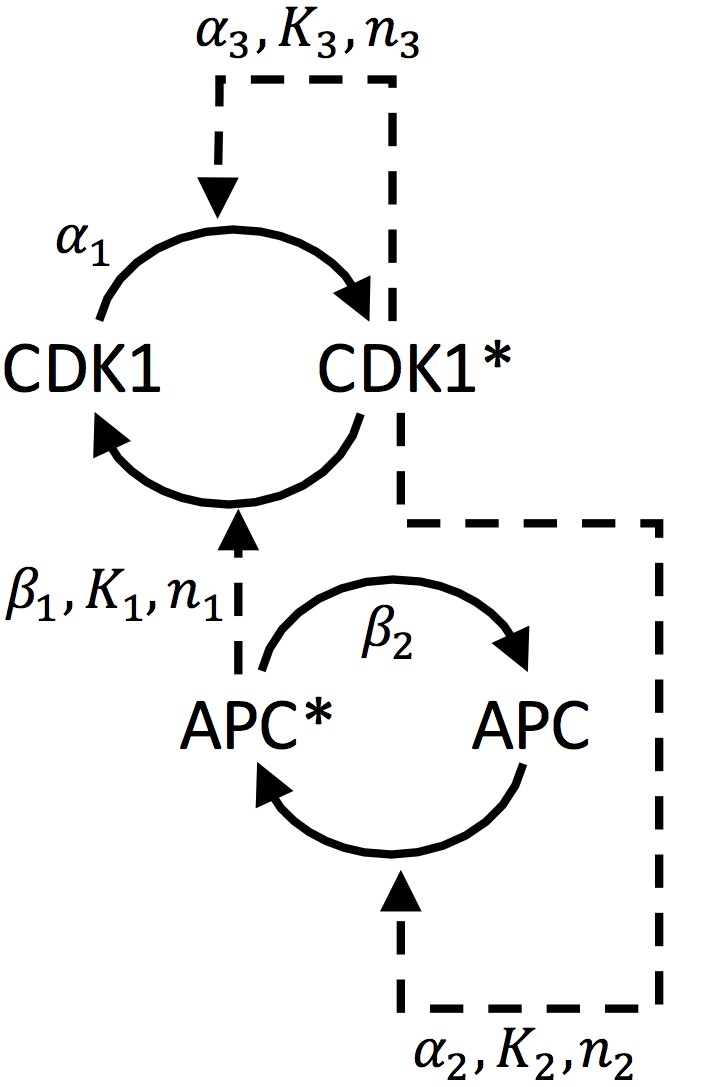
\includegraphics{CDK1-APC-model.png}
\end{center}

\begin{parts}
\part[10] Write a set of differential equations for the model (Hint: You only need two equations.)
\part[10] Make a schematic diagram that indicates positive and negative feedbacks. (Hint: There should be two nodes.)
\part[10]Take the parameter values to be $\alpha_1=0.02$, $\alpha_2=\alpha_3=3$, $\beta_1=3$, $\beta_2=1$, $K_1=K_2=K_3=0.5$, and $n_1=n_2=n_3=3$. Plot the nullclines, flow fields, and a representative set of trajectories in the phase plane. Describe the dynamics. 
\part[10] Change the parameter to $n_1=n_2=n_3=8$ while keeping everything else the same. Plot the nullclines, flow fields, and a representative set of trajectories in the phase plane. Describe the dynamics.
\part[10] What happens to the stability of the fixed points when as the parameters changed?
Comment on the eigenvalues of the Jacobian matrix that describe the system. (Extra points for numerically determining the eigen values for the two cases.)

\end{parts}	
\end{question}

\newpage

\question (50 points) Consider a simple network of two interacting proteins X and Y that form the following network, where $X$, $Y$, and $XY$ represent the amounts of X, Y and their complex XY respectively:
\begin{align*}
X&\xrightarrow{\lambda_X}X+1 & X &\xrightarrow{X}X-1 \\
Y&\xrightarrow{\lambda_Y}Y+1 & Y  &\xrightarrow{Y}Y - 1 \\
X,Y,XY&\xrightarrow{c\cdot X\cdot Y}X-1,Y-1,XY +1 &XY&\xrightarrow{XY} XY-1
%\emptyset\xrightarrow{\lambda_X}&X\xrightarrow{1}\emptyset \\
%\emptyset\xrightarrow{\lambda_Y}&Y\xrightarrow{1}\emptyset \\
%X+Y\xrightarrow{c}&XY\xrightarrow{1}\emptyset
\end{align*}
Protein X is a transcription factor that acts as a repressor for the expression of a third protein Z, which we will add to the model in part (d). Protein Y binds to X to form a complex XY that is transcriptionally inactive. The production rates $\lambda_X$ and $\lambda_Y$ can be taken to be 50 molecules/s and 30 molecules/s respectively, and $c$ is 50 /molecule/s.
\begin{parts}
\part[10] Compute the mean steady state values of $X$, $Y$, and $XY$ and compare these with the expected mean values of $X$ and $Y$ in the absence of complexation. How would you describe Y's regulation of X?
\part[10] Compute the steady state variances in $X$, $Y$, and $XY$, and compare them to what would be expected from a simple birth-death process with the same mean value.
\part[5] Compare the observed probability that $X<4$ from your stochastic trajectory with the expected probability from a simple birth-death process with the same mean value of X. How is this result related to your findings in (b)? 
\part[10] Now consider an additional component Z, whose production is regulated in an all-or-none fashion by X:
\begin{align*}
    Z &\xrightarrow{f(X)} Z+ 1 & Z &\xrightarrow{Z}Z-1,
\end{align*}
where $f(X)=\lambda_Z \Theta(X<4)$ and $\Theta$ is the Heaviside function, which evaluates to 1 if the argument is True and 0 if the argument is False. Take $\lambda_Z$ to be 1000 molecules/second. Compute a stochastic trajectory of the system of about 1000 time units and plot the amount of Z vs. time. Describe your observations.
(\emph{Hint:} In case you are trying to use BNGL for problem 2 on the Long Answer section, here is a \href{https://canvas.pitt.edu/files/17420689/download?download_frd=1}{BNGL model} that implements a Heaviside function for a stochastic model along with a \href{https://canvas.pitt.edu/files/17420690/download?download_frd=1}{Jupyter notebook} that can run it).

\part[10] Suppose that Z is itself a transcription factor that induces expression of genes that switches the cell to a different phenotype. We will refer to the phenotype with low Z expression as A and the phenotype with high Z expression as B. Assume that phenotype B persists as long as $Z>4$. Run a trajectory of at least 20,000 time units and determine the distribution of lifetimes for each phenotype. Plot the resulting distributions and compute the mean lifetime of each state. For each state what type of distribution is observed?
\part[5] What are the biological implications of the distributions for each state?
\end{parts}
\end{questions}



\end{document}
